\documentclass{beamer}
\usepackage{fancybox}
\usepackage{tikz}
\usetikzlibrary{shapes, arrows.meta, positioning}
% \usetikzlibrary{arrows.meta,
%                 chains,
%                 positioning, 
%                 shadows.blur, shapes.arrows}
              
\usetheme{Madrid}

\title{Logical Neural Networks}
\author{Robert Hoehndorf}
\date{\today}

\begin{document}

\frame{\titlepage}

\begin{frame}
\frametitle{Overview}
\begin{itemize}
\item aim: represent logical formulas {\em in the neural network
    structure}
  \begin{itemize}
  \item neural networks encode ``syntax''
  \end{itemize}
\item compositional neural network structure
\item disentangled representation
\item no exact truth values: maintain upper and lower bounds for
  propositions
\end{itemize}
\end{frame}

\begin{frame}
  \frametitle{Overview 2}
  \begin{itemize}
  \item neurons have bidirectional relationship with each neighbor
    \begin{itemize}
    \item omnidirectional inference
    \end{itemize}
  \item enable computation of exact entailments
  \end{itemize}
\end{frame}

\begin{frame}
\frametitle{The Basic Setup -- the Logic}
\begin{itemize}
    \item The underlying logic is fuzzy (assigning values to the
      logical syntax) and weighted (formulas have logical connectors
      associated with them).
    \item Inputs are initial truth value bounds $[L,U]$ for formulas
      and/or atoms.
    \begin{itemize}
        \item e.g., atom \texttt{inClass(student1)} has a truth value
          in $[0.9, 1.0]$.
        \item e.g., formula \texttt{inClass(student1) AND
            inClass(student2)} has a truth value in $[0.8,1.0]$.
    \end{itemize}
    \item Outputs are also truth value bounds for formulas or atoms.
    \item The formulas are known ahead of time.
    \item The weights and biases associated with formulas are not.
    \item The underlying logical connectors (fuzzy version of AND, OR,
      quantifiers, etc.) not only depend on the fuzzy values of the
      formulas being combined, but also the weight and bias of the
      operators.
    \item Note that the same operator will have a different weight and
      bias for each formula it appears in.
\end{itemize}
\end{frame}

\begin{frame}
\frametitle{The Basic Setup -- Inference}
\begin{itemize}
    \item Input to inference:
    \begin{itemize}
        \item Set of formulas.
        \item Initial truth bounds for each atom and formula.
        \item Bias and weight for each formula (connector).
    \end{itemize}
    \item Output:
    \begin{itemize}
        \item Final truth bounds for each formula and atom.
    \end{itemize}
    \item Authors propose an upward--downward pass through the logic
      (this is different from forward--backward pass used in gradient
      descent).
    \item The algorithm propagates truth values from atoms to the
      formula (upward) and from the formulas to the atoms (downward)
      until convergence.
\end{itemize}
\end{frame}

\begin{frame}
\frametitle{The Basic Setup -- Learning}
\begin{itemize}
    \item Neural architecture is derived directly from the {\em a
        priori} known formulas.
    \item Historical inputs and outputs used as samples during the
      training process.
    \item Loss function depends not only on standard ML metrics (e.g.,
      MSE) but also the number of inconsistencies (neurons associated
      with a truth bound where $L>U$).
    \item The functions used to combine formulas are differentiable
      with respect to the weights.
    \item The forward pass of the learning process can be done with
      the inference algorithm (which is essentially a fixpoint
      operator).
\end{itemize}
\end{frame}

\begin{frame}
\frametitle{The Logic}
\begin{itemize}
    \item Both atoms and formulas are associated with reals in the
      interval $[0,1]$.
    \item In practice, LNNs only provide information about a bound on
      the real-value associated with the atoms and formulas.
    \item This allows for uncertainty.
    \item The authors propose a threshold $\alpha$ for assigning
      truth, falsehood, or uncertainty in the result.
\end{itemize}
\bigskip % Adds some space before the table
\begin{tabular}{lcccc}
\hline
\textbf{Bounds} & \textbf{Unknown} & \textbf{True} & \textbf{False} &
                                                                      \textbf{Contradiction} \\
\hline
  Upper & $[\alpha, 1]$ & $[\alpha, 1]$ & $[0, 1 - \alpha]$ & Lower $>$ Upper \\
  Lower & $[0, 1 - \alpha]$ & $[\alpha, 1]$ & $[0, 1 - \alpha]$ & \\
\hline
\end{tabular}
\end{frame}

\begin{frame}
\frametitle{Weighted Real-Valued Logic}
\begin{itemize}
    \item The logic is also weighted -- components of logical formulas
      are weighted, hence they can be decomposed.
    \item This allows for inference.
    \item This decomposition allows the logic to be directly
      translated into a neural structure via the syntax tree of each
      formula.
\end{itemize}
\end{frame}


\begin{frame}
  \frametitle{Example}
  \centerline{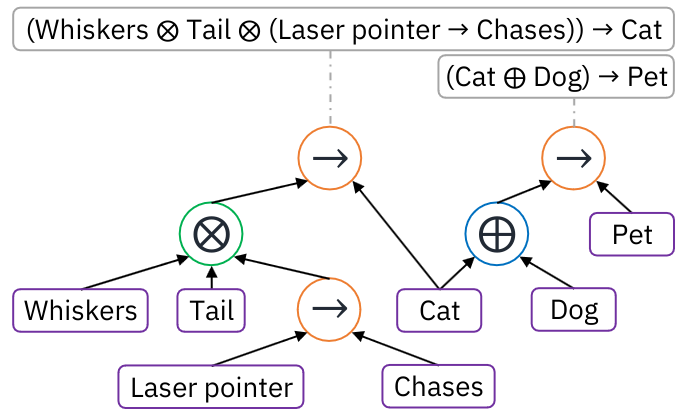
\includegraphics[width=.8\textwidth]{lnn1.png}}
\end{frame}

\begin{frame}
  \frametitle{Activation function}
  \centerline{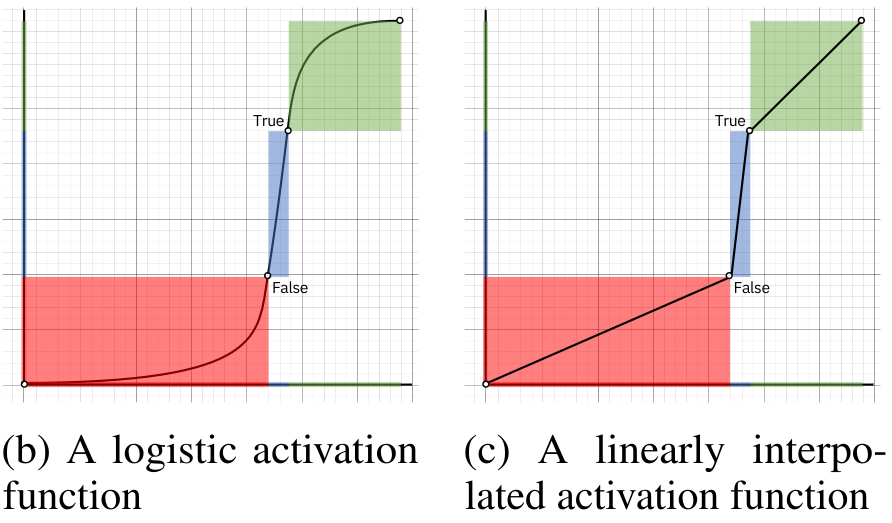
\includegraphics[width=.6\textwidth]{lnn2.png}}
  \begin{itemize}
  \item The authors are open about a variety of activation functions and
    settings of $\alpha$, but do make arguments for a ``tailored
    activation function'' in the paper.
  \end{itemize}
\end{frame}

\begin{frame}
\frametitle{The Strategy Behind LNN Inference}
\begin{itemize}
    \item Define correct proof rules with respect to the logic.
    \item Define how the bounds change based on atoms and negations
      are concluded from proof rules.
    \item Prove a minimal required set of proof rules based on the
      direction of inference (atoms to formulas vs. formulas to
      atoms).
    \item Put it all together in an algorithm that can be proven
      correct based on the above items.
\end{itemize}
\end{frame}

\begin{frame}
\frametitle{LNN Proof Rules and Tightening of Bounds}
\begin{itemize}
  \item The basic proof rules – these are not the precise definitions
    used in the algorithm, but rather showing the classical case to
    which LNN inference corresponds.
  \begin{itemize}
    \item $x, x \rightarrow y \vdash y$ (modus ponens)
    \item $\neg y, x \rightarrow y \vdash \neg x$ (modus tollens)
    \item $x, \neg (x \land y) \vdash \neg y$ (conjunctive syllogism)
    \item $\neg x, x \lor y \vdash y$ (disjunctive syllogism)
  \end{itemize}
  \item As LNN is not classical, it is tightening bounds based on the
    inference rules. This occurs as it concludes a literal (either an
    atom or its negation).
  % \item The bounds computations for $\neg$ are trivial:
  % \begin{itemize}
  %   \item $L_{\neg x} \geq \neg U_x = 1 - U_x, L_x \geq \neg U_{\neg x} = 1 - U_{\neg x},$
  %   \item $U_{\neg x} \leq \neg L_x = 1 - L_x, U_x \leq \neg L_{\neg x} = 1 - L_{\neg x}.$
  % \end{itemize}
\end{itemize}
\end{frame}

\begin{frame}
\frametitle{Weighted Nonlinear Conjunctions}
\begin{itemize}
    \item Used for logical AND, $\land$
    \item Defined as:
    \[ \beta (\bigotimes_{i \in I} x_i^{\otimes w_i}) = f\left(\beta -
        \sum_{i \in I} w_i (1 - x_i)\right) \]
    \item Here, \( f \) is a function from \( \mathbb{R} \) to \( [0,
      1] \), satisfying \( f(1 - x) = 1 - f(x) \).
    \item The bias term \( \beta \geq 0 \), weights \( w_i \geq 0 \),
      and inputs \( x_i \in [0, 1] \).
\end{itemize}
\end{frame}

\begin{frame}
\frametitle{Weighted Nonlinear Disjunctions}
\begin{itemize}
    \item Used for logical OR.
    \item Defined as:
    \[ \beta (\bigoplus_{i \in I} x_i^{\oplus w_i}) = f\left(1 - \beta + \sum_{i \in I} w_i x_i\right) \]
    \item \( \beta \) and weights \( w_i \) establish a hyperplane in relation to inputs \( x_i \), but clamped to \( [0, 1] \).
\end{itemize}
\end{frame}

\begin{frame}
\frametitle{Activation Functions and Bias Terms}
\begin{itemize}
    \item For \( f(x) = \max\{0, \min\{1, x\}\} \), the activation functions resemble the rectified linear unit (ReLU).
    \item These functions are also akin to the Łukasiewicz t- and s-norms.
    \item Bias term \( \beta \) allows classically equivalent formulas \( x \rightarrow y \), \( \neg y \rightarrow \neg x \), and \( \neg x \oplus y \) to be equivalent in this logic by adjusting \( \beta \).
\end{itemize}
\end{frame}

\begin{frame}
\frametitle{Weighted Nonlinear Residuum}
\begin{itemize}
    \item Used for logical implication.
    \item Defined as:
    \[ \beta (x^{\otimes w_x} \rightarrow y^{\oplus w_y}) = f\left(1 - \beta + w_x(1 - x) + w_y y\right) \]
    \item The residuum uses \( \otimes \) in the antecedent (AND-like weighting) and \( \oplus \) in the consequent (OR-like weighting).
    \item It behaves differently based on the value of \( \beta \), adapting to various logical equivalences.
\end{itemize}
\end{frame}

\begin{frame}
\frametitle{Behavior of the Weighted Nonlinear Residuum}
\begin{itemize}
    \item Most disjunction-like when \( \beta = 1 \).
    \item Most \( x \rightarrow y \)-like when \( \beta = w_y \).
    \item Most \( \neg y \rightarrow \neg x \)-like when \( \beta = w_x \).
\end{itemize}
\end{frame}


\begin{frame}
\frametitle{Inference Rules}
\framesubtitle{Introduction to Bounds}
In the context of Weighted Nonlinear Logic:
\begin{itemize}
\item \(L\) and \(U\) denote the lower and upper bounds for the
  truth values of neurons corresponding to formulas.
\item For example, \(L_{x \rightarrow y}\) represents the lower-bound
  truth value for the formula \(x \rightarrow y\).
\item \(U_x\) is the upper bound for just the truth value of \(x\).
\end{itemize}
\end{frame}

\begin{frame}
\frametitle{Inference Rules}
\framesubtitle{Bounds Computations for Negation}
The computations for negation (\(\neg\)) are straightforward:
\begin{align*}
L_{\neg x} & \geq 1 - U_x, \\
L_x & \geq 1 - U_{\neg x}, \\
U_{\neg x} & \leq 1 - L_x, \\
U_x & \leq 1 - L_{\neg x}.
\end{align*}
These inequalities allow for the possibility of tighter bounds from
other sources.
\end{frame}

\begin{frame}
\frametitle{Inference Rules}
\framesubtitle{Tighter Bounds and Sources}
\begin{itemize}
\item Tighter bounds for each value may be derived from other sources.
\item For instance, both \(y\) and \(x \rightarrow \neg y\) can inform
  \(L_{\neg y}\); LNNs use the tighter of the two.
\end{itemize}
\end{frame}

\begin{frame}
\frametitle{Inference Rules}
\framesubtitle{Nonlinear Transformation in Weighted Logic}
In the logic of LNNs:
\begin{itemize}
    \item Use the transformation \(\beta (x^{ \otimes w_x} \rightarrow
      y^{\oplus w_y}) = \beta ((1 - x)^{ \oplus w_x} \oplus y^{ \oplus
        w_y})\) and $\beta \left( \bigotimes_{i \in I} x_i^{\otimes w_i} \right) = 1 - \beta \left( \bigoplus_{i \in I} (1 - x_i)^{\oplus w_i} \right)$

    \item Allows to define a single set of inference rules to cover
      all connectives.
\end{itemize}
\end{frame}

\begin{frame}
\frametitle{Inference Rules}
\framesubtitle{Upward and Downward Bounds Computations}
The computations for upward bounds:
\begin{itemize}
\item $L_{\bigoplus i} x_i \geq \beta \left( \bigoplus_{i \in I}
    L^{\oplus w_i}_{x_i} \right)$
\item $U_{\bigoplus i} x_i \leq \beta \left( \bigoplus_{i \in I}
    U^{\oplus w_i}_{x_i} \right)$ 
\end{itemize}
The computations for downward bounds:
\begin{itemize}
\item \begin{align*}
L_{x_i} \geq \frac{\beta}{w_i} \left( \bigotimes_{\substack{j \neq i}} (1 - U_{x_j})^{\otimes \frac{w_j}{w_i}} \right) \otimes L^{\otimes \frac{1}{w_i}}_{\bigoplus i} x_i \quad \text{if } L_{\bigoplus i} x_i > 1 - \alpha, \text{ else } 0
\end{align*}
\item \begin{align*}
U_{x_i} \leq \frac{\beta}{w_i} \left( \bigotimes_{\substack{j \neq i}} (1 - L_{x_j})^{\otimes \frac{w_j}{w_i}} \right) \otimes U^{\otimes \frac{1}{w_i}}_{\bigoplus i} x_i \quad \text{if } U_{\bigoplus i} x_i < \alpha, \text{ else } 1
\end{align*}
\end{itemize}
Here, \(\alpha\) is a threshold to address potential divergent
behaviors at $L_{\bigoplus i} x_i \leq 1 - \alpha$ and $U_{\bigoplus
  i} x_i \geq \alpha$
\end{frame}

\begin{frame}
\frametitle{Inference Rules}
\framesubtitle{ReLU Case and Inference Implications}
In the ReLU case where \(f(x) = \max\{0, \min\{1, x\}\}\):
\begin{itemize}
    \item The function \(x \oplus y\) can return $1$ for many
      combinations of \(x\) and \(y\).
    \item Specifically, whenever \(w_x x + w_y y \geq \beta\).
    \item If \(U_{\oplus i} x_i = 1\), we cannot infer an upper bound
      for any \(x_i\).
\end{itemize}
\end{frame}

\begin{frame}
  \frametitle{LNN Inference: Upward--Downward Algorithm}
  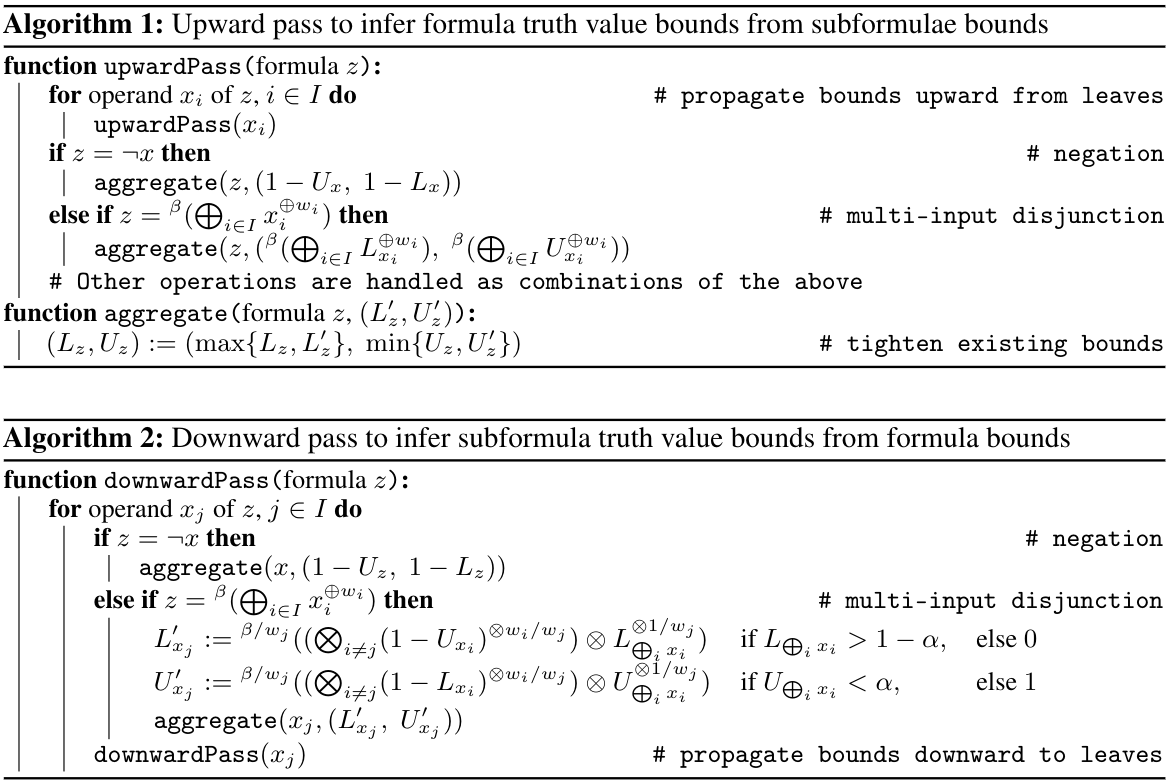
\includegraphics[width=\textwidth]{lnn3.png}
\end{frame}

\begin{frame}
\frametitle{Overall Strategy}
\begin{itemize}
    \item Use gradient descent to find weights, employing normal
      back-propagation and the aforementioned inference process for
      the forward pass.
    \item The loss function combines normal metrics (e.g., MSE) with a
      count of inconsistent neurons.
\end{itemize}
\end{frame}

\begin{frame}
\frametitle{Key Issues to Consider}
\begin{itemize}
    \item Parameters \(w\) and \(b\) must be set in such a way that
      classical logic outcomes for the operators behave as
      expected. For example, if either proposition \(a\) or \(b\) has
      a value of 1, the disjunction should always result in 1.
    \item Balancing learning parameters that fit the model with the
      interpretability of the model is crucial.
\end{itemize}
\end{frame}

\begin{frame}
\frametitle{Objective Function with Constraints}
\begin{itemize}
    \item The parameter-learning problem is framed as an optimization
      problem with constraints to ensure reasonable parameter
      settings.
    \item Objective:
    \[ \min_{B,W} E(B, W) + \sum_{k \in N} \max\{0, L_{B,W,k} - U_{B,W,k}\} \]
    \item Subject to constraints for every \(k \in N\), \(i \in I_k\):
    \[ \alpha \cdot w_{ik} - \beta_k + 1 \geq \alpha, \quad w_{ik} \geq 0 \]
    \[ \sum_{i \in I_k} (1 - \alpha) \cdot w_{ik} - \beta_k + 1 \leq 1
      - \alpha, \quad \beta_k \geq 0 \] 
    \item \(E(B,W)\) represents the traditional loss function.
    \item The summation is designed to reduce the number of inconsistencies.
\end{itemize}
\end{frame}

\begin{frame}
\frametitle{Optimization for Classical Behavior in Weighted Nonlinear Logic}
\begin{itemize}
    \item Weighted nonlinear logic behaves classically for classical
      inputs when optimized with the given objective and constraints.
    \item Constraints ensure:
    \begin{enumerate}
        \item Disjunctions return True if any input is true (\( \alpha
          \cdot w_{ik} - \beta_k + 1 \geq \alpha \)).
        \item Disjunctions return False if all inputs are false (\(
          \sum_{i \in I_k} (1 - \alpha) \cdot w_{ik} - \beta_k + 1
          \leq 1 - \alpha \)).
    \end{enumerate}
    \item Loss function \(E\) often includes NN learning objectives
      such as mean-square error.
    \item Contradiction loss penalizes the total contradiction
      observed in the system.
\end{itemize}
\end{frame}

\begin{frame}
\frametitle{Tailored Activation Function for Disjunction}
\begin{itemize}
    \item For disjunction with \(\beta = 1\), a tailored activation
      function \(f_w\) is utilized.
    \item \(f_w\) is a linear interpolation between four critical points:
    \begin{enumerate}
        \item \((0, 0)\) for the origin,
        \item \((x_F, 1 - \alpha)\) for the start of the True region,
        \item \((x_T, \alpha)\) for the threshold between intermediate and True,
        \item \((x_{\text{max}}, 1)\) for the maximum input value.
    \end{enumerate}
\end{itemize}
\end{frame}

\begin{frame}
\frametitle{Defining the Tailored Activation Function}
The function \(f_w(x)\) is defined piecewise:
\begin{itemize}
    \item \(f_w(x) = x \cdot \frac{1 - \alpha}{x_F}\) if \(0 \leq x
      \leq x_F\),
    \item \(f_w(x) = (x - x_F) \cdot \frac{2\alpha - 1}{x_T - x_F} + 1
      - \alpha\) if \(x_F < x < x_T\),
    \item \(f_w(x) = (x - x_T) \cdot \frac{1 - \alpha}{x_{\text{max}}
        - x_T} + \alpha\) if \(x_T \leq x \leq x_{\text{max}}\).
\end{itemize}
\end{frame}

\begin{frame}
\frametitle{Critical Points and Classicality}
\begin{itemize}
    \item \(x_F = \sum_{i \in I} w_i \cdot (1 - \alpha)\), \(x_T =
      w_{\text{max}} \cdot \alpha\), \(x_{\text{max}} = \sum_{i \in I}
      w_i\).
    \item This configuration ensures classical inputs yield classical
      results without constraints.
    \item The definition of \(x_T\) allows for weights to approach
      zero without affecting \(f_w\)'s effectiveness.
\end{itemize}
\end{frame}

\begin{frame}
\frametitle{Implications of Tailored Activation Function}
\begin{itemize}
    \item Monotonic linear interpolation ensures gradients are large
      and reliable across all regions.
    \item The parameter \(\alpha\) serves as a mechanism to control
      the system's classicality:
    \begin{itemize}
    \item Smaller \(\alpha\) values result in more classical behavior.
    \end{itemize}
\end{itemize}
\end{frame}

\begin{frame}
  \frametitle{Comparison to LTNs}
  \begin{itemize}
  \item no arbitrary queries (LTNs allow)
  \item symbolic explanations (not in LTNs)
  \item encode prior knowledge, constraints (same in LTNs)
  \item does not ensure consistency (same in LTNs)
  \item does not learn rules/formulas (same in LTNs)
  \item scalable (?)
  \end{itemize}
\end{frame}

\end{document}

%%% Local Variables:
%%% mode: latex
%%% coding: utf-8
%%% TeX-master: t
%%% eval: (TeX-run-style-hooks "beamer")
%%% End:
